\documentclass[tikz,border=8pt]{standalone}
\usepackage{amsmath}
\usepackage{amssymb}
\usepackage{tikz}
\usetikzlibrary{arrows.meta}

\begin{document}

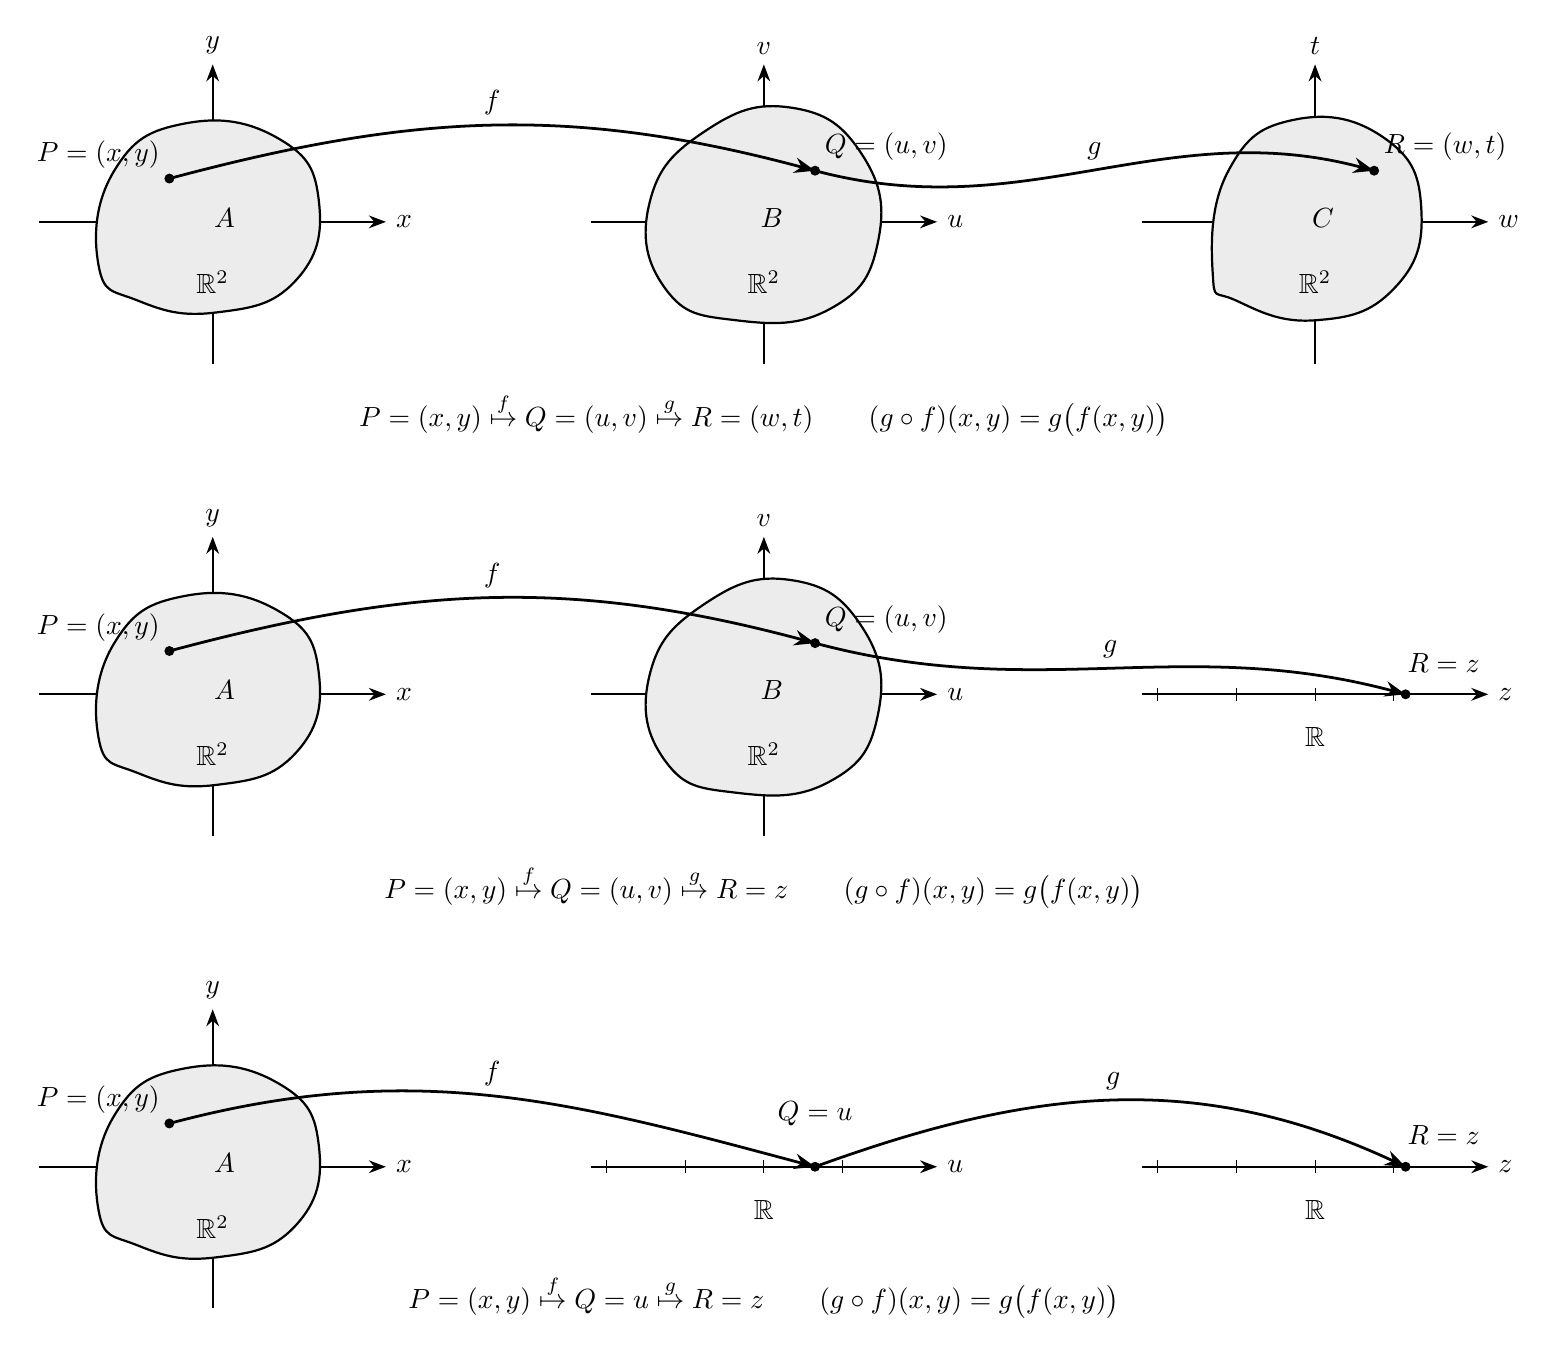
\begin{tikzpicture}[
    >=Stealth,
    axis/.style={
        ->,
        line width=0.7pt
    },
    mapping/.style={
        ->,
        line width=1pt
    }
]

% ============================================================
% 第一幅：R^2 -> R^2 -> R^2
% ============================================================

\begin{scope}[yshift=0cm]

    % 左侧坐标系
    \begin{scope}[xshift=0cm]
        \draw[axis]
            (-2.2,0) -- (2.2,0)
            node[right] {$x$};

        \draw[axis]
            (0,-1.8) -- (0,2.0)
            node[above] {$y$};

        \filldraw[
            fill=gray!15,
            draw=black,
            thick
        ]
        plot[smooth cycle, tension=0.8]
        coordinates {
            (-1.45,-0.55)
            (-1.25,0.65)
            (-0.35,1.25)
            (0.85,1.05)
            (1.35,0.25)
            (1.05,-0.75)
            (0.05,-1.15)
            (-0.95,-1.00)
        };

        \node at (0.15,0.05) {$A$};

        \coordinate (P1) at (-0.55,0.55);
        \fill (P1) circle (1.8pt);

        \node[above left] at (P1)
            {$P=(x,y)$};

        \node[below=5mm] at (0,0)
            {$\mathbb{R}^{2}$};
    \end{scope}

    % 中间坐标系
    \begin{scope}[xshift=7cm]
        \draw[axis]
            (-2.2,0) -- (2.2,0)
            node[right] {$u$};

        \draw[axis]
            (0,-1.8) -- (0,2.0)
            node[above] {$v$};

        \filldraw[
            fill=gray!15,
            draw=black,
            thick
        ]
        plot[smooth cycle, tension=0.8]
        coordinates {
            (-1.25,-0.85)
            (-1.45,0.25)
            (-0.75,1.15)
            (0.35,1.45)
            (1.25,0.85)
            (1.45,-0.25)
            (0.85,-1.10)
            (-0.35,-1.25)
        };

        \node at (0.1,0.05) {$B$};

        \coordinate (Q1) at (0.65,0.65);
        \fill (Q1) circle (1.8pt);

        \node[above right] at (Q1)
            {$Q=(u,v)$};

        \node[below=5mm] at (0,0)
            {$\mathbb{R}^{2}$};
    \end{scope}

    % 右侧坐标系
    \begin{scope}[xshift=14cm]
        \draw[axis]
            (-2.2,0) -- (2.2,0)
            node[right] {$w$};

        \draw[axis]
            (0,-1.8) -- (0,2.0)
            node[above] {$t$};

        \filldraw[
            fill=gray!15,
            draw=black,
            thick
        ]
        plot[smooth cycle, tension=0.8]
        coordinates {
            (-1.30,-0.65)
            (-1.10,0.65)
            (-0.25,1.30)
            (0.90,1.05)
            (1.35,0.15)
            (1.00,-0.85)
            (0.00,-1.25)
            (-1.00,-1.00)
        };

        \node at (0.1,0.05) {$C$};

        \coordinate (R1) at (0.75,0.65);
        \fill (R1) circle (1.8pt);

        \node[above right] at (R1)
            {$R=(w,t)$};

        \node[below=5mm] at (0,0)
            {$\mathbb{R}^{2}$};
    \end{scope}

    % 映射箭头
    \draw[mapping]
        (P1)
        to[out=15,in=165]
        node[above] {$f$}
        (Q1);

    \draw[mapping]
        (Q1)
        to[out=-15,in=165]
        node[above] {$g$}
        (R1);

    % 函数等式
    \node at (7,-2.45)
        {$P=(x,y)\overset{f}{\mapsto}Q=(u,v)\overset{g}{\mapsto}R=(w,t)\qquad(g\circ f)(x,y)=g\bigl(f(x,y)\bigr)$};

\end{scope}


% ============================================================
% 第二幅：R^2 -> R^2 -> R
% ============================================================

\begin{scope}[yshift=-6cm]

    % 左侧坐标系
    \begin{scope}[xshift=0cm]
        \draw[axis]
            (-2.2,0) -- (2.2,0)
            node[right] {$x$};

        \draw[axis]
            (0,-1.8) -- (0,2.0)
            node[above] {$y$};

        \filldraw[
            fill=gray!15,
            draw=black,
            thick
        ]
        plot[smooth cycle, tension=0.8]
        coordinates {
            (-1.45,-0.55)
            (-1.25,0.65)
            (-0.35,1.25)
            (0.85,1.05)
            (1.35,0.25)
            (1.05,-0.75)
            (0.05,-1.15)
            (-0.95,-1.00)
        };

        \node at (0.15,0.05) {$A$};

        \coordinate (P2) at (-0.55,0.55);
        \fill (P2) circle (1.8pt);

        \node[above left] at (P2)
            {$P=(x,y)$};

        \node[below=5mm] at (0,0)
            {$\mathbb{R}^{2}$};
    \end{scope}

    % 中间坐标系
    \begin{scope}[xshift=7cm]
        \draw[axis]
            (-2.2,0) -- (2.2,0)
            node[right] {$u$};

        \draw[axis]
            (0,-1.8) -- (0,2.0)
            node[above] {$v$};

        \filldraw[
            fill=gray!15,
            draw=black,
            thick
        ]
        plot[smooth cycle, tension=0.8]
        coordinates {
            (-1.25,-0.85)
            (-1.45,0.25)
            (-0.75,1.15)
            (0.35,1.45)
            (1.25,0.85)
            (1.45,-0.25)
            (0.85,-1.10)
            (-0.35,-1.25)
        };

        \node at (0.1,0.05) {$B$};

        \coordinate (Q2) at (0.65,0.65);
        \fill (Q2) circle (1.8pt);

        \node[above right] at (Q2)
            {$Q=(u,v)$};

        \node[below=5mm] at (0,0)
            {$\mathbb{R}^{2}$};
    \end{scope}

    % 右侧数轴
    \begin{scope}[xshift=14cm]
        \draw[axis]
            (-2.2,0) -- (2.2,0)
            node[right] {$z$};

        \foreach \x in {-2,-1,0,1}
            \draw (\x,0.08) -- (\x,-0.08);

        \coordinate (R2) at (1.15,0);
        \fill (R2) circle (1.8pt);

        \node[above=4mm,right=-1mm] at (R2)
            {$R=z$};

        \node[below=3mm] at (0,0)
            {$\mathbb{R}$};
    \end{scope}

    % 映射箭头
    \draw[mapping]
        (P2)
        to[out=15,in=165]
        node[above] {$f$}
        (Q2);

    \draw[mapping]
        (Q2)
        to[out=-15,in=165]
        node[above] {$g$}
        (R2);

    % 函数等式
    \node at (7,-2.45)
        {$P=(x,y)\overset{f}{\mapsto}Q=(u,v)\overset{g}{\mapsto}R=z \qquad (g\circ f)(x,y)=g\bigl(f(x,y)\bigr)$};
\end{scope}


% ============================================================
% 第三幅：R^2 -> R -> R
% ============================================================

\begin{scope}[yshift=-12cm]

    % 左侧坐标系
    \begin{scope}[xshift=0cm]
        \draw[axis]
            (-2.2,0) -- (2.2,0)
            node[right] {$x$};

        \draw[axis]
            (0,-1.8) -- (0,2.0)
            node[above] {$y$};

        \filldraw[
            fill=gray!15,
            draw=black,
            thick
        ]
        plot[smooth cycle, tension=0.8]
        coordinates {
            (-1.45,-0.55)
            (-1.25,0.65)
            (-0.35,1.25)
            (0.85,1.05)
            (1.35,0.25)
            (1.05,-0.75)
            (0.05,-1.15)
            (-0.95,-1.00)
        };

        \node at (0.15,0.05) {$A$};

        \coordinate (P3) at (-0.55,0.55);
        \fill (P3) circle (1.8pt);

        \node[above left] at (P3)
            {$P=(x,y)$};

        \node[below=5mm] at (0,0)
            {$\mathbb{R}^{2}$};
    \end{scope}

    % 中间数轴
    \begin{scope}[xshift=7cm]
        \draw[axis]
            (-2.2,0) -- (2.2,0)
            node[right] {$u$};

        \foreach \x in {-2,-1,0,1}
            \draw (\x,0.08) -- (\x,-0.08);

        \coordinate (Q3) at (0.65,0);
        \fill (Q3) circle (1.8pt);

        \node[above=4mm] at (Q3)
            {$Q=u$};

        \node[below=3mm] at (0,0)
            {$\mathbb{R}$};
    \end{scope}

    % 右侧数轴
    \begin{scope}[xshift=14cm]
        \draw[axis]
            (-2.2,0) -- (2.2,0)
            node[right] {$z$};

        \foreach \x in {-2,-1,0,1}
            \draw (\x,0.08) -- (\x,-0.08);

        \coordinate (R3) at (1.15,0);
        \fill (R3) circle (1.8pt);

        \node[above=4mm,right=-1mm] at (R3)
            {$R=z$};

        \node[below=3mm] at (0,0)
            {$\mathbb{R}$};
    \end{scope}

    % R^2 -> R
    \draw[mapping]
        (P3)
        to[out=15,in=165]
        node[above] {$f$}
        (Q3);

    % R -> R，弓形避开数轴
    \draw[mapping]
        (Q3)
        to[out=20,in=155]
        node[above] {$g$}
        (R3);

    % 函数等式
    \node at (7,-1.65)
        {$P=(x,y)\overset{f}{\mapsto}Q=u\overset{g}{\mapsto}R=z\qquad (g\circ f)(x,y)=g\bigl(f(x,y)\bigr)$};

\end{scope}

\end{tikzpicture}

\end{document}